\chapter{État de l'art des techniques de recommandation}
\chaptermark{Techniques}
\minitoc
\newpage

\section{Recommandation aléatoire}
Bien avant la technologie du machine learning, la recommandation était basée sur des propositions aléatoires des articles au client. Certaines fois les articles les plus populaires sont recommandés. Ce qui pose un problème de personnalisation des produits pour chaque client. Un article peut être populaire mais ne pourra intéresser certains,cela peut devenir contre productif si on se base sur ce type de recommandation. C’est l’exemple d’une recommandation d’articles dépendant du sexe du client.

\section{Recommandation Personnalisée}
Cette méthode consiste à recommander un produit sur la base de ses achats précédents, de ses motifs de recherche. Elle vise à proposer au mieux les produits beaucoup plus successible d'intéresser le client. Mais dans ce cas, si le client n’avait jamais effectué d’achat ou pas assez de commande, il reste difficile de recommander d’autres articles susceptibles de l'intéresser.

\section{Recommandation Objet (Content-Based filtering CB)}
Dans ce type de recommandation, on se base sur les caractéristiques que présente le produit et faire la recommandation sur les caractéristiques des produits que le client a déjà choisi (soit recommander des produits similaires à celui choisi dans le panier). \\
Pour construire le modèle basé sur la méthode du Content Based, il faut tokenizer les caractéristiques des produits ensuite appliquer les méthodes du TF-IDF. Ceci permet d’augmenter l’importance ou la fréquence des mots clés du produits et de réduire les mots inutiles. \\
Le problème de cette approche de recommandation Objet, est qu'elle nécessite une connaissance profonde des produits à recommander puisqu'elle est basée sur la description ou le nom du produit.\\
- Exemple:
Considérons deux produits qui ont dans leur description les informations suivantes:\\
 	P1: “Pneu souple de qualité”\\
P2: “Pneu de qualité”\\
Pour connaître la similarité entre ces deux produits on peut appliquer la méthode de similarité basée sur le calcule du cosinus. Tout d’abord, on calcule la fréquence des mots clés que contient chaque description, ensuite on projette chaque produit dans un repère n-dimensionnel. Deux vecteurs P1 et P2 de cet espace ainsi constitués sont similaires si et seulement si  le cosinus de leur angle est petit.

\begin{figure}[h]
\begin{center}
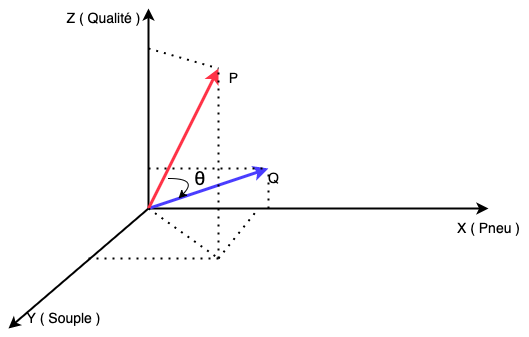
\includegraphics[width=15cm,height=8cm]{images/cosin_similarity.png}
\caption[Projection des produits]{Projection des produits}
\label{monlabel}
\end{center}
\end{figure}

$$\cos(\theta )={\mathbf {P} \cdot \mathbf {Q} \over \|\mathbf {P} \|\|\mathbf {Q} \ |}$$
 $$={\frac {\sum \limits _{i=1}^{n}{P_{i}Q_{i}}}{{\sqrt {\sum \limits _{i=1}^{n }{P_{i}^{2}}}}{\sqrt {\sum \limits _{i=1}^{n}{Q_{i}^{2}}}}}}$$
 
 \section{Recommandation Sociale (Collaborative Filtering CF – Context Aware)}
 Basée sur le comportement ou le vote des clients, le modèle du Collaborative Filtering utilise les avis clients sur des produits pour les recommander à d’autres utilisateurs.\\

On distingue plusieurs approches de collaborative filtering:\\
\subsection{Memory-based CF}
Cette approche se base sur les votes, cliques sur lequel il faut établir une corrélation entre les produits ou entre les utilisateurs afin de recommander un produit quelconque à un utilisateur qui ne l'a jamais vu. Dans ce cas plus précis, les produits recommandés sont ceux achetés par les utilisateurs les plus proches.
\subsection{La Matrice de Factorisation}
Cette méthode vise à factoriser la matrice de base obtenue en considérant le vote de chaque client pour chaque article. Cette factorisation permet de simplifier la matrice de base en deux matrices (Client et Article) dont le produit matriciel est similaire à la matrice de base.

$$M = U x I$$

\begin{figure}[h]
\begin{center}
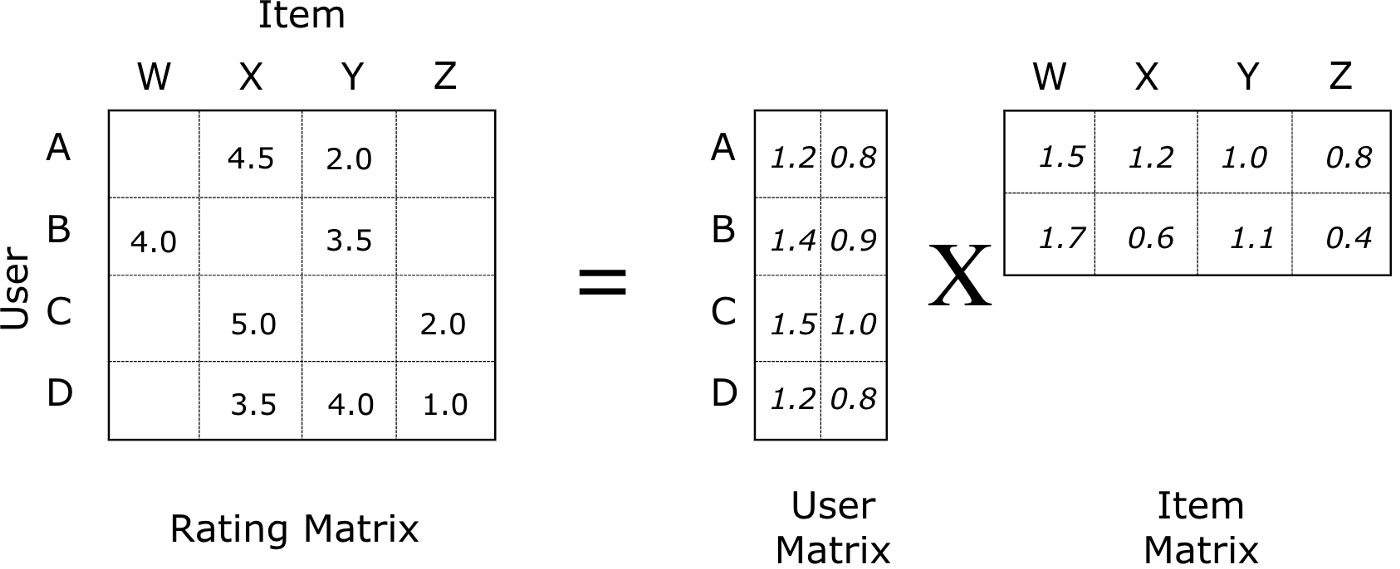
\includegraphics[width=17cm,height=8cm]{images/factorisation_matrix.png}
\caption[Décomposition de la matrice]{Décomposition de la matrice}
\label{monlabel}
\end{center}
\end{figure}

\begin{figure}[h]
\begin{center}
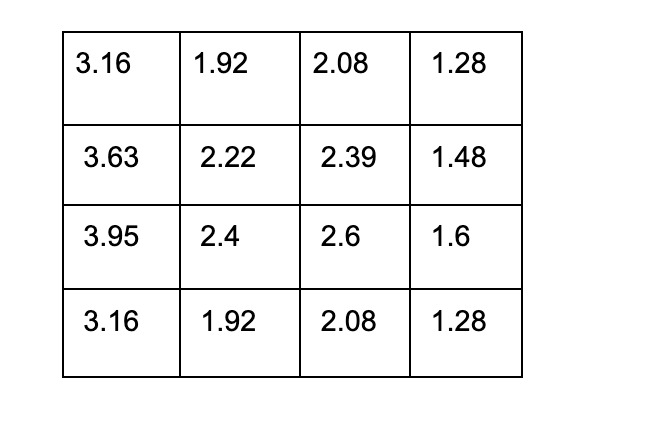
\includegraphics[width=15cm,height=8cm]{images/factorisation_result.jpeg}
\caption[Matrice produit]{Matrice produit}
\label{monlabel}
\end{center}
\end{figure}

\subsection{Neural Collaborative Filtering (NFC)}
Il est possible d’appliquer le modèle de réseau de neurone au problème de recommandation. A partir de la matrice des clients et des articles, on envoie en entrée du réseau un encodage de vecteur unitaire du client et de l’article. A l'intérieur le vecteur est connecté à plusieurs couches comme par exemple le perceptron multicouche. 
\newpage
\begin{figure}[h]
\begin{center}
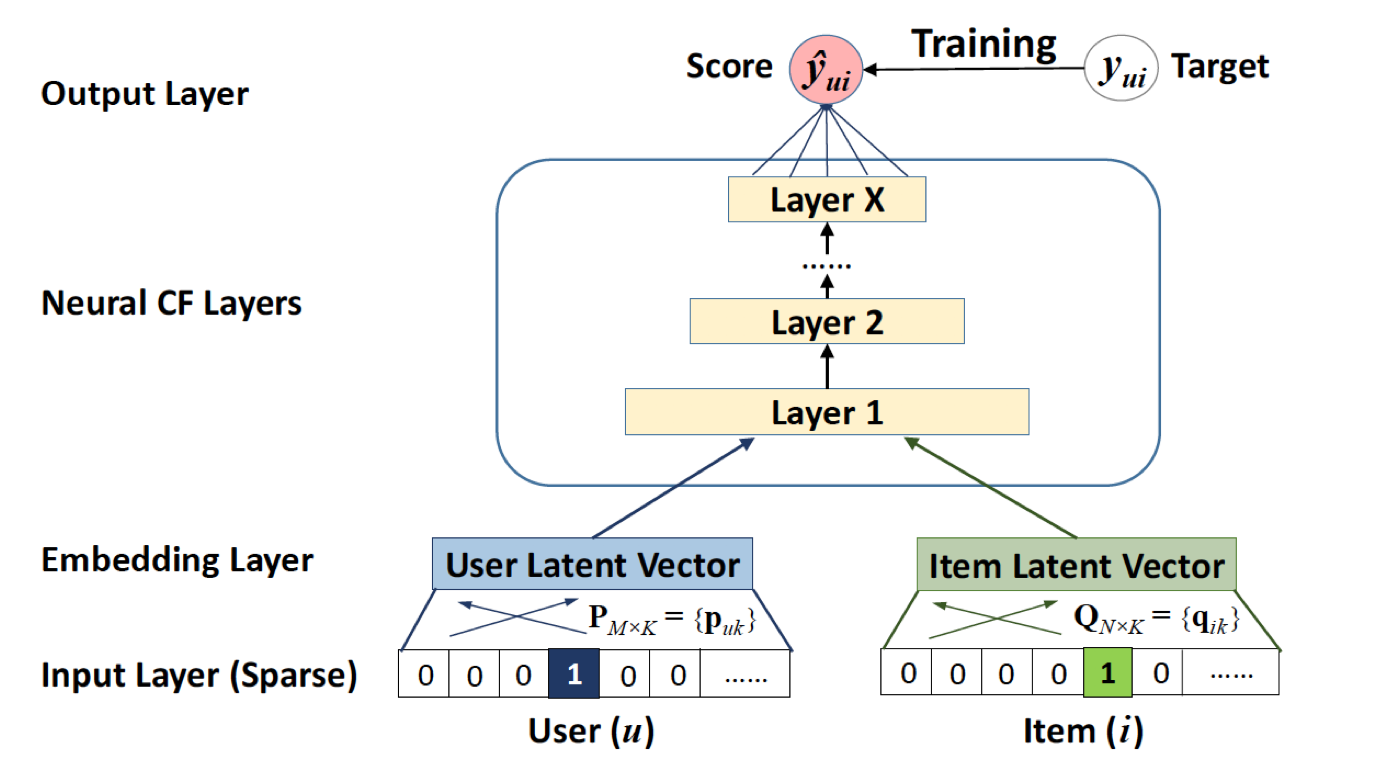
\includegraphics[width=15cm,height=8cm]{images/neural_cf.png}
\caption[Neural Colaborative Filtering, https://towardsdatascience.com/neural-collaborative-filtering-96cef1009401]{Neural Colaborative Filtering, https://towardsdatascience.com/neural-collaborative-filtering-96cef1009401}
\label{monlabel}
\end{center}
\end{figure}
Cette méthode généralise la méthode de factorisation de matrice.
Premièrement, en remplaçant la couche interne avec une unique couche de multiplication, on se retrouve avec le schéma ci-dessous.
\begin{figure}[h]
\begin{center}
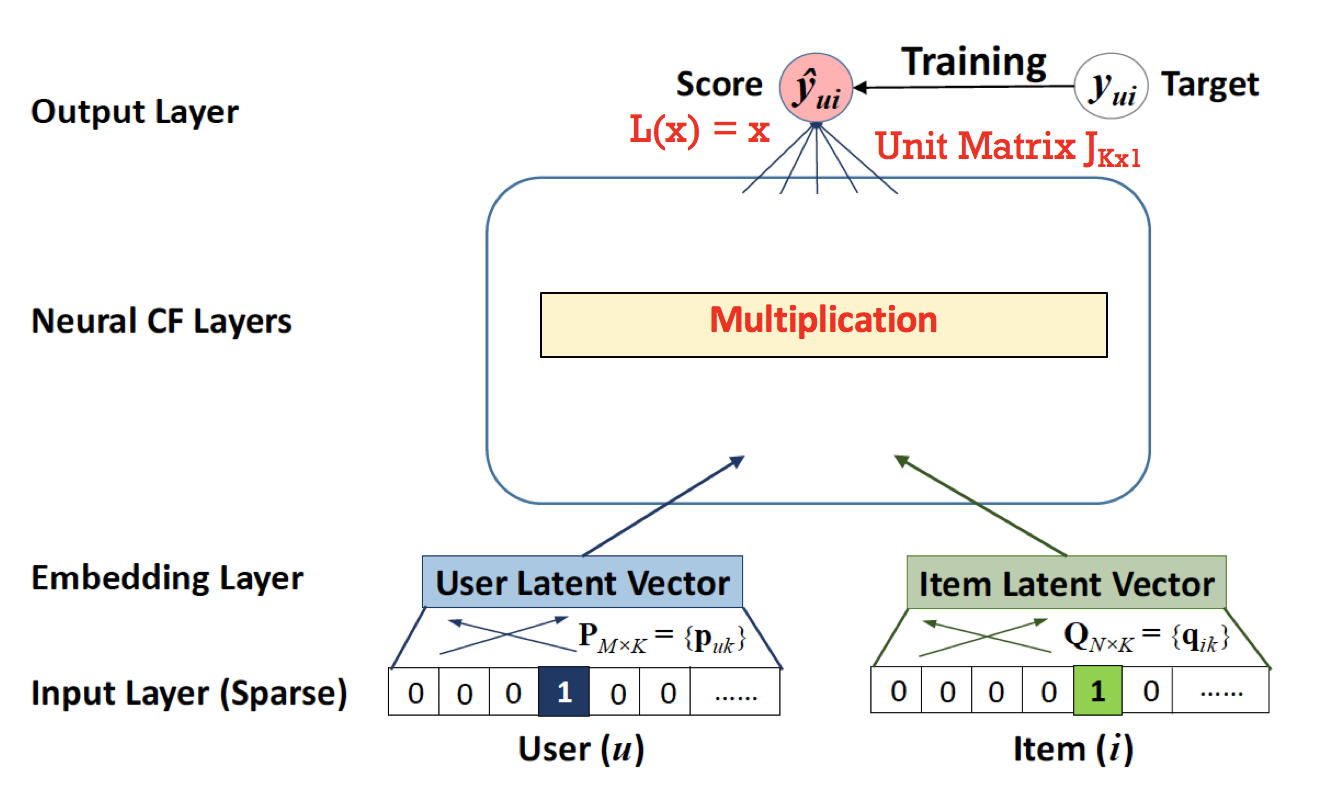
\includegraphics[width=15cm,height=8cm]{images/nfc_multiplication.png}
\caption[Généralisation du NFC, https://towardsdatascience.com/neural-collaborative-filtering-96cef1009401]{Généralisation du NFC, https://towardsdatascience.com/neural-collaborative-filtering-96cef1009401}
\label{monlabel}
\end{center}
\end{figure}

Ensuite on initialise le poids de la couche de sortie à une matrice J dont toutes les valeurs sont égales à 1 et une fonction d’activation linéaire L. 
$$L(x) = x$$
\newpage
\begin{figure}[h]
\begin{center}
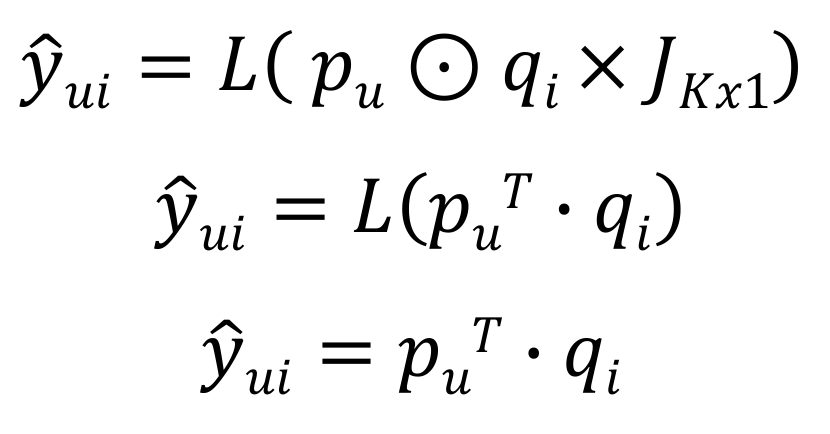
\includegraphics[width=8cm,height=4cm]{images/nfc_proof.png}
\caption[]{}
\label{monlabel}
\end{center}
\end{figure}
Ce qui revient exactement à une décomposition en un produit de deux matrices. On conclut que la méthode de matrice factorisation est un cas particulier du Neuron Collaborative Filtering.

\subsection{LSTM: Long Short Term Memory}
LSTM: Long Short Term Memory est un algorithme de la famille des réseaux de neurone récurrent (RNN)
\begin{itemize}
  	\item Réseau de Neurone récurrent:\\
  		Un réseau de neurone récurrent est une succession d’état des neurones qui gagnent des informations du précédent état. Chaque état a une entrée input X(t) et une sortie output h(t) définissant la prédiction. La partie A est une couche de neurones dont les informations sont propagées à l’état suivant.
  		\begin{figure}[h]
\begin{center}
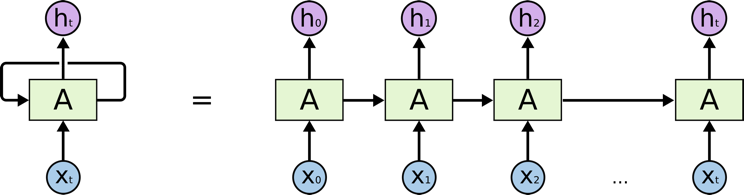
\includegraphics[width=16cm,height=5cm]{images/rnn_steps.png}
\caption[Etats du RNN: https://towardsdatascience.com/understanding-lstm-and-its-quick-implementation-in-keras-for-sentiment-analysis-af410fd85b47]{Etats du RNN: https://towardsdatascience.com/understanding-lstm-and-its-quick-implementation-in-keras-for-sentiment-analysis-af410fd85b47}
\label{monlabel}
\end{center}
\end{figure}
	\item Cas particulier du LSTM:\\
Dans chaque couche, il existe quatre portes qui contrôlent le comportement de l’information.

	\begin{itemize}
  		\item Input Gate:\\
Cette porte contrôle s’il faut écrire le vecteur d'entrée dans la mémoire du LSTM c(t) ou non . Elle comporte une couche de sigmoïde.
\item Forget Gate:\\
Cette porte a une couche de sigmoïde qui déterminent s’il faut supprimer l’information de la mémoire du LSTM c(t).
\item Candidate Gate:\\
Cette porte détermine quelle information écrire dans la mémoire c(t) à partir de la couche de tan(h).
	\item Output Gate:\\
Dans cette porte, une fonction sigmoïde aussi détermine quelle information sort en sortie de la l’état caché. 

	\end{itemize}
	  		\begin{figure}[h]
\begin{center}
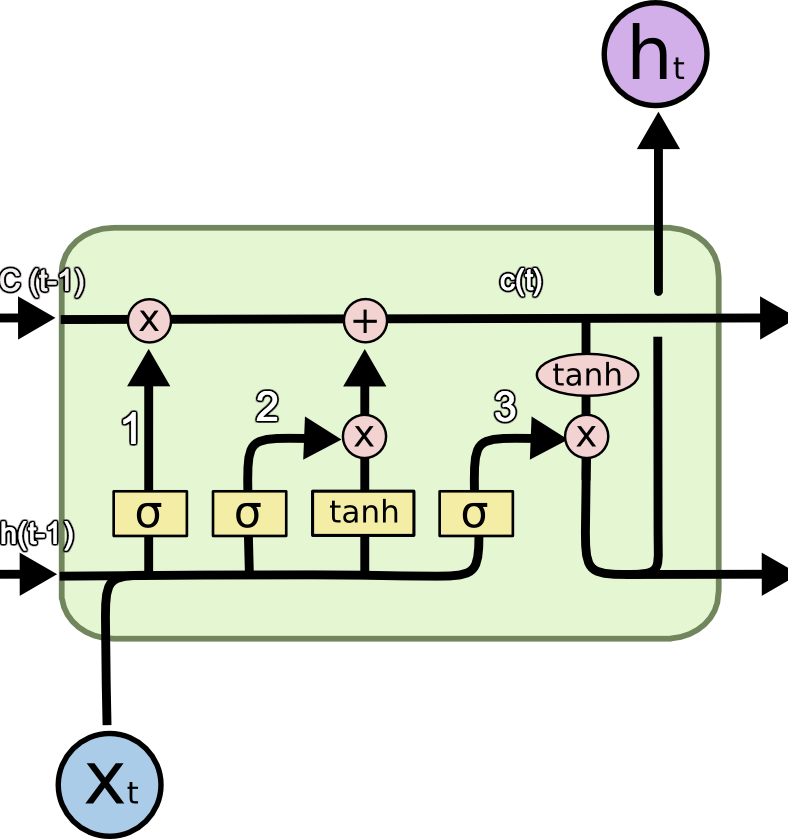
\includegraphics[width=12cm,height=10cm]{images/lstm_layer.png}
\caption[Couche du LSTM: https://towardsdatascience.com/understanding-lstm-and-its-quick-implementation-in-keras-for-sentiment-analysis-af410fd85b47]{Couche du LSTM: https://towardsdatascience.com/understanding-lstm-and-its-quick-implementation-in-keras-for-sentiment-analysis-af410fd85b47}
\label{monlabel}
\end{center}
\end{figure}


\end{itemize}
$X$: Scaling of information\\
$+$ : Ajout d' information\\
$\sigma$: Couche de Sigmoïde (valeurs {0, 1} donc pour faire oublier ou garder l’information)\\
$tan(h)$: Couche de tangente (pour faire maintenir le gradient non nul plus longtemp)\\
$h(t-1)$ : Sortie du précedent LSTM\\
$c(t-1)$ : Memoire du précedent LSTM\\
$X(t)$ : Vecteur d'entrer en cours\\
$c(t)$ : Nouvelle nise à jour du mémoire\\
$h(t)$ : Sortie en cours\\